\documentclass[a4paper, 11pt]{article}
\usepackage[top=3cm, bottom=3cm, left=2.5cm, right=2.5cm]{geometry}
\usepackage{amsmath}
\usepackage{amsfonts}
\usepackage{graphicx}
\usepackage{psfrag}
\usepackage[utf8]{inputenc}
\usepackage[T1]{fontenc}
\usepackage[french]{babel}
\usepackage{hyperref}

\title{Rapport : Factures}
\author{Pierre BONNEFOY, Ilyes ZEGHDALLOU, Alexandre MARINE, Aloys LANA}


\begin{document}


\maketitle

\tableofcontents

\newpage
\section{Définition du Projet}
Pour ce projet, nous avons choisit de nous lancer dans la création d'un logiciel d'analyse des Factures. Notre positionnement sera le suivant : nous sommes une entreprise tierce qui fournit un service à des clients (professionnels ou particuliers). Le client peut rentrer ses factures sur notre système et ensuite peut executer deux actions sur celle ci :
\begin{enumerate}
    \item Demander le montant total de toutes ses factures sur une période donnée ou/et provenant d'une entreprise spécifique.
    \item Demander la liste des entreprises qui lui ont vendu un produit spécifique.
\end{enumerate}

\section{Modélisation de la Base de Données}
A CHANGER ALEX DOIT ENVOYER UNE AUTRE VERSION
    \begin{center}
    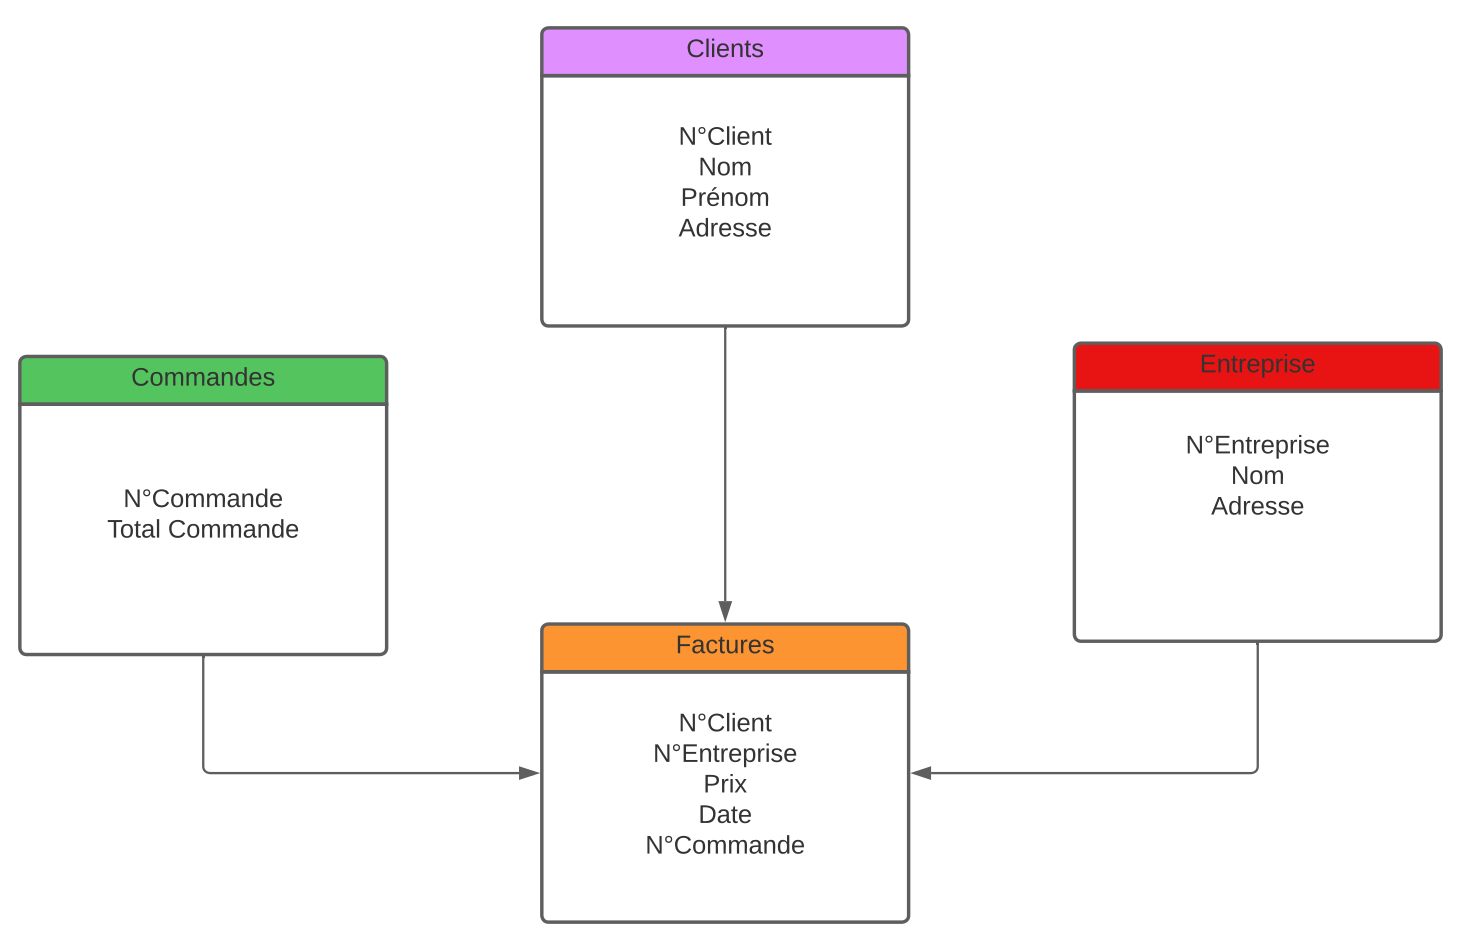
\includegraphics[scale=0.3]{schema_bdd.png}
    \end{center}

\section{Modélisations du Message 1}
    \subsection{Intitulé du Message}
        \subsubsection{Requête} 
        L'application métier demande à la Base de Données de lui envoyer le total de toutes les factures d'une entreprise cible et/ou d'une période cible.
        \subsubsection{Réponse}
        La Base de Données renvoie la somme de tous les totaux de chaque factures correspondant aux contraintes énoncées dans la requête.
    \subsection{Format JSON}
        \subsubsection{Requête}
        
        \subsubsection{Réponse}
        \begin{verbatim}
            {
            "reponse" : {
                        "type" : 1,
                        "to" : "appMetier",
                        "from" : "bdd",
                        "id_discussion" : 1,
                        "nom_client" : "Proton",
                        "total" : 21
                        }
            }
        \end{verbatim}
\section{Modélisations du Message 2}
    \subsection{Intitulé du Message}
        \subsubsection{Requête} 
        L'application métier demande à la Base de Données de lui envoyer la liste des entreprises lui ayant vendu un produit spécifique.
        \subsubsection{Réponse}
        La Base de Données renvoie la liste de toutes les entreprises lui ayant vendu ce produit.
    \subsection{JSON Schema}
        \subsubsection{Requête}
        \begin{verbatim}
            {
            "title": Reponse
            
            "properties":{
                
            }
            }
        \end{verbatim}
    
    
    \subsection{Format JSON}
        \subsubsection{Requête}
            
        \subsubsection{Reponse}
        \begin{verbatim}
            {
            "reponse" : {
                        "type" : 1,
                        "to" : "appMetier",
                        "from" : "bdd",
                        "id_discussion" : 1,
                        "nom_client" : "Proton",
                        "liste_entreprises" : ["giroud", "mbappe", "messi"]
                        }
            }
        \end{verbatim}

\section{Choix des technologies}
Pour ce projet, nous avons choisit d'utiliser le langage Python au vu de sa simplicité d'utilisation et de sa diversité de bibliothèques permettant de nous facilité le travail.\\
En voici la liste :
\begin{enumerate}
    \item json : une bibliothèque permettant de traiter et de générer des fichiers JSON.
    \item tkinter : une bibliothèque graphique qui nous a permit de réalisé l'interface utilisateur.
\end{enumerate}

\section{Tâches et répartition}
    \subsection{Analyse de Fichiers}
    \begin{center}
    \begin{tabular}{|c|c|c|c|}
        \hline
        Enoncé de la Tâche & Personne assignée & Etat & Priorité\\
        \hline
        \hline
        Determiner les informations à relevé  & Pierre BONNEFOY & Finit & HAUTE \\
        \hline
        Repérage des Mots-Clés & Pierre BONNEFOY & Finit & HAUTE  \\
        \hline
        Développer une procédure de relevé & Pierre BONNEFOY & Finit & HAUTE  \\
        \hline
        Adaptation à plusieurs types de factures & Pierre BONNEFOY & En Cours & HAUTE  \\
        \hline
        Enregistrer dans la Base de Données & Pierre BONNEFOY & En Cours & HAUTE  \\
        \hline
    \end{tabular}
    \end{center}

    \subsection{Communication de la Base de Données}
    \begin{center}
    \begin{tabular}{|c|c|c|c|}
        \hline
        Enoncé de la Tâche & Personne assignée & Etat & Priorité\\
        \hline
        \hline
        Créer une Base de Données  & Alexandre MARINE & En Cours & HAUTE \\
        \hline
        Gérer l'accés a la Base de Données  & Alexandre MARINE & En Cours & HAUTE \\
        \hline
        Réception des requête de AM  & Alexandre MARINE & En Cours & HAUTE \\
        \hline
        Générer la réponse en JSON  & Alexandre MARINE & En Cours & HAUTE \\
        \hline
    \end{tabular}
    \end{center}

    \subsection{Génération des requêtes depuis l'application métier}
    \begin{center}
    \begin{tabular}{|c|c|c|c|}
        \hline
        Enoncé de la Tâche & Personne assignée & Etat & Priorité\\
        \hline
        \hline
        Creer le formulaire du message 1  & Ilyes ZEGHDALLOU & En Cours & HAUTE \\
        \hline
        Creer le formulaire du message 2  & Ilyes ZEGHDALLOU & En Cours & HAUTE \\
        \hline
        Génération du fichier JSON de la requête  & Ilyes ZEGHDALLOU & En Cours & HAUTE \\
        \hline
    \end{tabular}
    \end{center}

    \subsection{Réception des Réponses et Affichage coté Application Métier}
    \begin{center}
    \begin{tabular}{|c|c|c|c|}
        \hline
        Enoncé de la Tâche & Personne assignée & Etat & Priorité\\
        \hline
        \hline
        Scruter le Dossier de Simulation du réseau  & Aloys LANA & Finit & HAUTE \\
        \hline
        Récuperer les données du fichier JSON  & Aloys LANA & Finit & HAUTE \\
        \hline
        Afficher les résultats  & Aloys LANA & En Cours & HAUTE \\
        \hline
        Supprimer les anciens messages  & Aloys LANA & En Cours & HAUTE \\
        \hline
    \end{tabular}
    \end{center}


\section{Problèmes Rencontrés}
    \subsection{Analyse des documents}

    \subsection{Base de Données}

\end{document}

